\protect\hyperlink{main-nav}{≡} \protect\hyperlink{close-nav}{×}

\hypertarget{section-2.8-curve-sketching}{%
\section{Section 2.8: Curve
Sketching}\label{section-2.8-curve-sketching}}

This section examines some of the interplay between the shape of the
graph of \textbackslash{}(f\textbackslash{}) and the behavior of
\textbackslash{}(f'\textbackslash{}). If we have a graph of
\textbackslash{}(f\textbackslash{}), we will see what we can conclude
about the values of \textbackslash{}(f'\textbackslash{}). If we know
values of \textbackslash{}(f'\textbackslash{}), we will see what we can
conclude about the graph of \textbackslash{}(f\textbackslash{}). We will
also utilize the information from \textbackslash{}(f''\textbackslash{})
that we learning in the last section.

To view this video please enable JavaScript, and consider upgrading to a
web browser that \href{http://videojs.com/html5-video-support/}{supports
HTML5 video}

\hypertarget{first-derivative-information}{%
\subsection{First Derivative
Information}\label{first-derivative-information}}

\hypertarget{definitions}{%
\paragraph{Definitions}\label{definitions}}

The function \textbackslash{}(f(x)\textbackslash{}) is
\textbf{increasing} on \textbackslash{}((a,b)\textbackslash{}) if
\textbackslash{}(a \textbackslash{}lt x\_1 \textbackslash{}lt x\_2
\textbackslash{}lt b\textbackslash{}) implies \textbackslash{}(f( x\_1 )
\textbackslash{}lt f( x\_2 )\textbackslash{}).

The function \textbackslash{}(f(x)\textbackslash{}) is
\textbf{decreasing} on \textbackslash{}((a,b)\textbackslash{}) if
\textbackslash{}(a \textbackslash{}lt x\_1 \textbackslash{}lt x\_2
\textbackslash{}lt b\textbackslash{}) implies \textbackslash{}(f( x\_1 )
\textbackslash{}gt f( x\_2 )\textbackslash{}).

Graphically, \textbackslash{}(f\textbackslash{}) is \textbf{increasing}
(decreasing) if, as we move from left to right along the graph of
\textbackslash{}(f\textbackslash{}), the height of the graph
\textbf{increases} (decreases).

These same ideas make sense if we consider
\textbackslash{}(h(t)\textbackslash{}) to be the height (in feet) of a
rocket at time \textbackslash{}(t\textbackslash{}) seconds. We naturally
say that the rocket is rising or that its height is increasing if the
height \textbackslash{}(h(t)\textbackslash{}) increases over a period of
time, as \textbackslash{}(t\textbackslash{}) increases.

\hypertarget{example-1}{%
\paragraph{Example 1}\label{example-1}}

List the intervals on which the function shown is increasing or
decreasing.

\begin{figure}
\centering
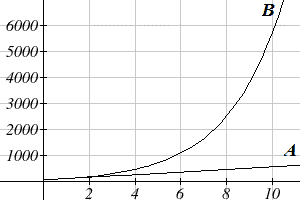
\includegraphics{images/image072.png}
\caption{}
\end{figure}

\textbackslash{}(f\textbackslash{}) is increasing on the intervals
{[}0,1{]}, {[} 2,3{]} and {[}4,6{]}.

\textbackslash{}(f\textbackslash{}) is decreasing on {[}1,2{]} and
{[}6,8{]}.

On the interval {[}3,4{]} the function is not increasing or decreasing
-- it is constant.

\hypertarget{first-derivative-information-about-shape}{%
\paragraph{First Derivative Information about
Shape}\label{first-derivative-information-about-shape}}

For a function \textbackslash{}(f\textbackslash{}) which is
differentiable on an interval \textbackslash{}((a,b)\textbackslash{});

\begin{itemize}
\tightlist
\item
  if \textbackslash{}(f\textbackslash{}) is increasing on
  \textbackslash{}((a,b)\textbackslash{}), then \textbackslash{}(f'(x)
  \textbackslash{}geq 0\textbackslash{}) for all
  \textbackslash{}(x\textbackslash{}) in
  \textbackslash{}((a,b)\textbackslash{}).
\item
  if \textbackslash{}(f\textbackslash{}) is decreasing on
  \textbackslash{}((a,b)\textbackslash{}), then \textbackslash{}(f'(x)
  \textbackslash{}leq 0\textbackslash{}) for all
  \textbackslash{}(x\textbackslash{}) in
  \textbackslash{}((a,b)\textbackslash{}).
\item
  if \textbackslash{}(f\textbackslash{}) is constant on
  \textbackslash{}((a,b)\textbackslash{}), then \textbackslash{}(f'(x) =
  0\textbackslash{}) for all \textbackslash{}(x\textbackslash{}) in
  \textbackslash{}((a,b)\textbackslash{}).
\end{itemize}

\hypertarget{example-2}{%
\paragraph{Example 2}\label{example-2}}

The graph shows the height of a helicopter during a period of time.
Sketch the graph of the upward velocity of the helicopter,
\textbackslash{}( \textbackslash{}frac\{dh\}\{dt\} \textbackslash{}).

\begin{figure}
\centering
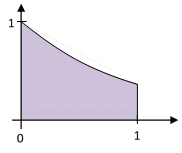
\includegraphics{images/image073.png}
\caption{}
\end{figure}

Notice that the \textbackslash{}( h(t)\textbackslash{}) has a local
maximum when \textbackslash{}(t = 2 \textbackslash{}) and
\textbackslash{}(t = 5\textbackslash{}), and so \textbackslash{}(v(2) =
0\textbackslash{}) and \textbackslash{}(v(5) = 0\textbackslash{}).
Similarly, \textbackslash{}(h(t)\textbackslash{}) has a local minimum
when \textbackslash{}(t = 3\textbackslash{}), so \textbackslash{}(v(3) =
0\textbackslash{}).

When \textbackslash{}(h\textbackslash{}) is increasing,
\textbackslash{}(v\textbackslash{}) is positive. When
\textbackslash{}(h\textbackslash{}) is decreasing,
\textbackslash{}(v\textbackslash{}) is negative.

Using this information, we can sketch a graph of \textbackslash{}(v(t) =
\textbackslash{}frac\{dh\}\{dt\}\textbackslash{}).

\begin{figure}
\centering
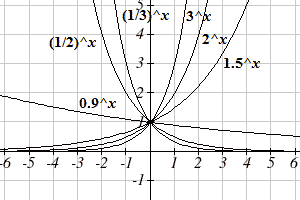
\includegraphics{images/image074.png}
\caption{}
\end{figure}

The next theorem is almost the converse of the First Shape Theorem and
explains the relationship between the values of the derivative and the
graph of a function from a different perspective. It says that if we
know something about the values of \textbackslash{}(f'\textbackslash{}),
then we can draw some conclusions about the shape of the graph of
\textbackslash{}(f\textbackslash{}).

\hypertarget{first-derivative-information-about-shape-part-2}{%
\paragraph{First Derivative Information about Shape (part
2)}\label{first-derivative-information-about-shape-part-2}}

For a function \textbackslash{}(f\textbackslash{}) which is
differentiable on an interval \textbackslash{}(I\textbackslash{});

\begin{itemize}
\tightlist
\item
  if \textbackslash{}(f'(x) \textbackslash{}gt 0\textbackslash{}) for
  all \textbackslash{}(x\textbackslash{}) in the interval
  \textbackslash{}(I\textbackslash{}), then
  \textbackslash{}(f\textbackslash{}) is increasing on
  \textbackslash{}(I\textbackslash{}).
\item
  if \textbackslash{}(f'(x) \textbackslash{}lt 0\textbackslash{}) for
  all \textbackslash{}(x\textbackslash{}) in the interval
  \textbackslash{}(I\textbackslash{}), then
  \textbackslash{}(f\textbackslash{}) is decreasing on
  \textbackslash{}(I\textbackslash{}).
\item
  if \textbackslash{}(f'(x) = 0\textbackslash{}) for all
  \textbackslash{}(x\textbackslash{}) in the interval
  \textbackslash{}(I\textbackslash{}), then
  \textbackslash{}(f\textbackslash{}) is constant on
  \textbackslash{}(I\textbackslash{}).
\end{itemize}

\hypertarget{example-3}{%
\paragraph{Example 3}\label{example-3}}

Use information about the values of \textbackslash{}(f'\textbackslash{})
to help graph \textbackslash{}(f(x) = x\^{}3 - 6x\^{}2 + 9x +
1\textbackslash{}).

\textbackslash{}(f'(x) = 3x\^{}2 - 12x + 9 = 3(x - 1)(x -
3)\textbackslash{}) so \textbackslash{}(f'(x) = 0\textbackslash{}) only
when \textbackslash{}(x = 1\textbackslash{}) or \textbackslash{}(x =
3\textbackslash{}). \textbackslash{}(f'\textbackslash{}) is a polynomial
so it is always defined.

The only critical numbers for \textbackslash{}(f\textbackslash{}) are
\textbackslash{}(x = 1\textbackslash{}) and \textbackslash{}(x =
3\textbackslash{}), and they divide the real number line into three
intervals: \textbackslash{}((-\textbackslash{}infty,
1)\textbackslash{}), \textbackslash{}((1,3)\textbackslash{}), and
\textbackslash{}((3, \textbackslash{}infty)\textbackslash{}). On each of
these intervals, the function is either always increasing or always
decreasing.

If \textbackslash{}(x \textbackslash{}lt 1\textbackslash{}), then
\textbackslash{}(f '(x) =\textbackslash{}) 3(negative number)(negative
number) \textbackslash{}(\textbackslash{}gt 0\textbackslash{}) so
\textbackslash{}(f\textbackslash{}) is increasing.

If \textbackslash{}(1 \textbackslash{}lt x \textbackslash{}lt
3\textbackslash{}), then \textbackslash{}(f'(x) =\textbackslash{})
3(positive number)(negative number) \textbackslash{}(\textbackslash{}lt
0\textbackslash{}) so f is decreasing.

If \textbackslash{}(x \textbackslash{}gt 3\textbackslash{}), then
\textbackslash{}(f'(x) =\textbackslash{}) 3(positive number)(positive
number) \textbackslash{}(\textbackslash{}gt 0\textbackslash{}) so
\textbackslash{}(f\textbackslash{}) is increasing.

Even though we don't know the value of
\textbackslash{}(f\textbackslash{}) anywhere yet, we do know a lot about
the shape of the graph of \textbackslash{}(f\textbackslash{}): as we
move from left to right along the
\textbackslash{}(x\textbackslash{})-axis, the graph of
\textbackslash{}(f\textbackslash{}) increases until \textbackslash{}(x =
1\textbackslash{}), then the graph decreases until \textbackslash{}(x =
3\textbackslash{}), and then the graph increases again. The graph of
\textbackslash{}(f\textbackslash{}) makes "turns" when
\textbackslash{}(x = 1\textbackslash{}) and \textbackslash{}(x =
3\textbackslash{}); it has a local maximum at \textbackslash{}(x =
1\textbackslash{}), and a local minimum at \textbackslash{}(x =
3\textbackslash{}).

\begin{figure}
\centering
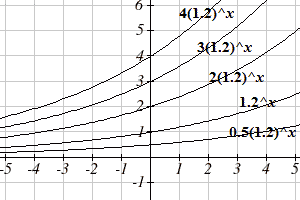
\includegraphics{images/image075.png}
\caption{}
\end{figure}

To plot the graph of \textbackslash{}(f\textbackslash{}), we still need
to evaluate \textbackslash{}(f\textbackslash{}) at a few values of
\textbackslash{}(x\textbackslash{}), but only at a very few values.
\textbackslash{}(f(1) = 5\textbackslash{}), and (1,5) is a local maximum
of \textbackslash{}(f\textbackslash{}). \textbackslash{}(f(3) =
1\textbackslash{}), and (3,1) is a local minimum of
\textbackslash{}(f\textbackslash{}). The resulting graph of
\textbackslash{}(f\textbackslash{}) is shown here.

\begin{figure}
\centering
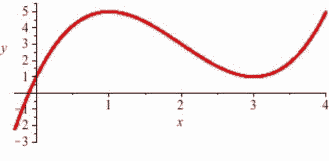
\includegraphics{images/image076.png}
\caption{}
\end{figure}

\hypertarget{second-derivative-information}{%
\subsection{Second Derivative
Information}\label{second-derivative-information}}

Until now, we've only used first derivative information, but we could
also use information from the second derivative to provide more
information about the shape of the function.

\hypertarget{second-derivative-information-about-shape}{%
\paragraph{Second Derivative Information about
Shape}\label{second-derivative-information-about-shape}}

\begin{itemize}
\tightlist
\item
  If \textbackslash{}(f\textbackslash{}) is concave up on
  \textbackslash{}((a,b)\textbackslash{}), then \textbackslash{}(f''(x)
  \textbackslash{}geq 0\textbackslash{}) for all
  \textbackslash{}(x\textbackslash{}) in
  \textbackslash{}((a,b)\textbackslash{}).
\item
  If \textbackslash{}(f\textbackslash{}) is concave down on
  \textbackslash{}((a,b)\textbackslash{}), then \textbackslash{}(f''(x)
  \textbackslash{}leq 0\textbackslash{}) for all
  \textbackslash{}(x\textbackslash{}) in
  \textbackslash{}((a,b)\textbackslash{}).
\end{itemize}

The converse of both of these are also true:

\begin{itemize}
\tightlist
\item
  If \textbackslash{}(f''(x) \textbackslash{}geq 0\textbackslash{}) for
  all \textbackslash{}(x\textbackslash{}) in
  \textbackslash{}((a,b),\textbackslash{}) then
  \textbackslash{}(f\textbackslash{}) is concave up on
  \textbackslash{}((a,b)\textbackslash{}).
\item
  If \textbackslash{}(f''(x) \textbackslash{}leq 0\textbackslash{}) for
  all \textbackslash{}(x\textbackslash{}) in
  \textbackslash{}((a,b),\textbackslash{}) then
  \textbackslash{}(f\textbackslash{}) is concave down on
  \textbackslash{}((a,b)\textbackslash{}).
\end{itemize}

To view this video please enable JavaScript, and consider upgrading to a
web browser that \href{http://videojs.com/html5-video-support/}{supports
HTML5 video}

\hypertarget{example-4}{%
\paragraph{Example 4}\label{example-4}}

Use information about the values of
\textbackslash{}(f''\textbackslash{}) to help determine the intervals on
which the function \textbackslash{}(f(x) = x\^{}3 - 6x\^{}2 + 9x +
1\textbackslash{}) is concave up and concave down.

For concavity, we need the second derivative: \textbackslash{}(
f'(x)=3x\^{}2-12x+9 \textbackslash{}), so \textbackslash{}( f''(x)=6x-12
\textbackslash{}).

To find possible inflection points, set the second derivative equal to
zero. \textbackslash{}( 6x-12=0 \textbackslash{}), so \textbackslash{}(x
= 2\textbackslash{}). This divides the real number line into two
intervals: \textbackslash{}( (-\textbackslash{}infty,2)
\textbackslash{}) and \textbackslash{}( (2,\textbackslash{}infty)
\textbackslash{}).

For \textbackslash{}(x \textbackslash{}lt 2\textbackslash{}), the second
derivative is negative (for example, \textbackslash{}(
f''(0)=6(0)-12=-12 \textbackslash{})), so
\textbackslash{}(f\textbackslash{}) is concave down. For
\textbackslash{}(x \textbackslash{}gt 2\textbackslash{}), the second
derivative is positive, so \textbackslash{}(f\textbackslash{}) is
concave up.

We could have incorporated this concavity information when sketching the
graph for the previous example, and indeed we can see the concavity
reflected in the graph shown.

To view this video please enable JavaScript, and consider upgrading to a
web browser that \href{http://videojs.com/html5-video-support/}{supports
HTML5 video}

\hypertarget{example-5}{%
\paragraph{Example 5}\label{example-5}}

Use information about the values of \textbackslash{}(f'\textbackslash{})
and \textbackslash{}(f''\textbackslash{}) to help graph
\textbackslash{}( f(x)=x\^{}\{2/3\} \textbackslash{}).

\textbackslash{}( f'(x)=\textbackslash{}frac\{2\}\{3\}x\^{}\{-1/3\}
\textbackslash{}). This is undefined at \textbackslash{}(x =
0\textbackslash{}).

\textbackslash{}( f''(x)=-\textbackslash{}frac\{2\}\{9\}x\^{}\{-4/3\}
\textbackslash{}). This is also undefined at \textbackslash{}(x =
0\textbackslash{}).

This creates two intervals: \textbackslash{}(x \textbackslash{}lt
0\textbackslash{}), and \textbackslash{}( x \textbackslash{}gt
0\textbackslash{}).

On the interval \textbackslash{}(x \textbackslash{}lt
0\textbackslash{}), we could test out a value like \textbackslash{}(x =
-1\textbackslash{}): \textbackslash{}{[}
f'(-1)=\textbackslash{}frac\{2\}\{3\}(-1)\^{}\{-1/3\}=-\textbackslash{}frac\{2\}\{3\}
\textbackslash{}{]} and \textbackslash{}{[}
f''(-1)=-\textbackslash{}frac\{2\}\{9\}(-1)\^{}\{-4/3\}=-\textbackslash{}frac\{2\}\{9\}.
\textbackslash{}{]}

\textbackslash{}( f'(x) \textbackslash{}) is negative and
\textbackslash{}( f''(x) \textbackslash{}) is negative, so we can
conclude that the function is decreasing and concave down on this
interval.

On the interval \textbackslash{}(x \textbackslash{}gt
0\textbackslash{}), we could test out a value like \textbackslash{}(x =
1\textbackslash{}): \textbackslash{}{[}
f'(1)=\textbackslash{}frac\{2\}\{3\}(1)\^{}\{-1/3\}=\textbackslash{}frac\{2\}\{3\}
\textbackslash{}{]} and \textbackslash{}{[}
f''(1)=-\textbackslash{}frac\{2\}\{9\}(1)\^{}\{-4/3\}=-\textbackslash{}frac\{2\}\{9\}.
\textbackslash{}{]}

\textbackslash{}( f'(x) \textbackslash{}) is positive and
\textbackslash{}( f''(x) \textbackslash{}) is negative, so we can
conclude that the function is increasing and concave down on this
interval.

We can also calculate that \textbackslash{}( f(0)=0 \textbackslash{}),
giving us a base point for the graph. Using this information, we can
conclude the graph must look like this:

\begin{figure}
\centering
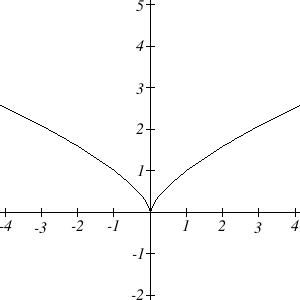
\includegraphics{images/image077.png}
\caption{}
\end{figure}

To view this video please enable JavaScript, and consider upgrading to a
web browser that \href{http://videojs.com/html5-video-support/}{supports
HTML5 video}

\hypertarget{sketching-without-an-equation}{%
\subsection{Sketching without an
Equation}\label{sketching-without-an-equation}}

Of course, graphing calculators and computers are great at graphing
functions. Calculus provides a way to illuminate what may be hidden or
out of view when we graph using technology. More importantly, calculus
gives us a way to look at the derivatives of functions for which there
is no equation given. We already saw the idea of this back in
\href{section2-3.php}{Section 2.3} where we sketched the derivative of
two graphs by estimating slopes on the curves.

We can summarize all the derivative information about shape in a table.

\hypertarget{summary-of-derivative-information-about-the-graph}{%
\paragraph{Summary of Derivative Information about the
Graph}\label{summary-of-derivative-information-about-the-graph}}

\begin{longtable}[]{@{}lllll@{}}
\toprule
\endhead
\textbackslash{}( f(x) \textbackslash{}) & Increasing & Decreasing &
Concave Up & Concave Down\tabularnewline
\textbackslash{}( f'(x) \textbackslash{}) & \textbackslash{}( +
\textbackslash{}) & \textbackslash{}( - \textbackslash{}) & Increasing &
Decreasing\tabularnewline
\textbackslash{}( f''(x) \textbackslash{}) & & & \textbackslash{}( +
\textbackslash{}) & \textbackslash{}( - \textbackslash{})\tabularnewline
\bottomrule
\end{longtable}

When \textbackslash{}(f'(x) = 0\textbackslash{}), the graph of
\textbackslash{}(f\textbackslash{}) may have a local max or min.

When \textbackslash{}(f''(x) = 0\textbackslash{}), the graph of
\textbackslash{}(f\textbackslash{}) may have an inflection point.

\hypertarget{example-6}{%
\paragraph{Example 6}\label{example-6}}

A company's bank balance, \textbackslash{}(B\textbackslash{}), in
millions of dollars, \textbackslash{}(t\textbackslash{}) weeks after
releasing a new product is shown in the graph below. Sketch a graph of
the marginal balance -- the rate at which the bank balance was changing
over time.

\begin{figure}
\centering
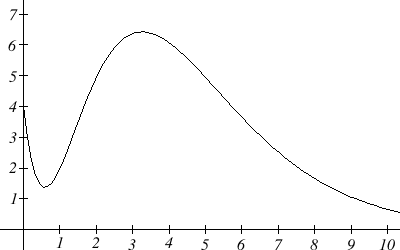
\includegraphics{images/image078.png}
\caption{}
\end{figure}

Notice that since the tangent line will be horizontal at about
\textbackslash{}(t = 0.6\textbackslash{}) and \textbackslash{}(t =
3.2\textbackslash{}), the derivative will be 0 at those points.

We can then identifying intervals on which the original function is
increasing or decreasing. This will tell us when the derivative function
is positive or negative.

\begin{longtable}[]{@{}lll@{}}
\toprule
\endhead
Interval & \textbackslash{}( B(t) \textbackslash{}) & \textbackslash{}(
B'(t) \textbackslash{})\tabularnewline
\textbackslash{}(0 \textbackslash{}lt t \textbackslash{}lt
0.6\textbackslash{}) & Decreasing & Negative\tabularnewline
\textbackslash{}( 0.6 \textbackslash{}lt t \textbackslash{}lt 3.2
\textbackslash{}) & Increasing & Positive\tabularnewline
\textbackslash{}( t \textbackslash{}gt 3.2 \textbackslash{}) &
Decreasing & Negative\tabularnewline
\bottomrule
\end{longtable}

There appear to be inflection points at about \textbackslash{}(t
=1.5\textbackslash{}) and \textbackslash{}(t = 5.5\textbackslash{}). At
these points, the derivative will be changing from increasing to
decreasing or vice versa, so the derivative will have a local max or min
at those points.

Looking at the intervals of concavity:

\begin{longtable}[]{@{}lll@{}}
\toprule
\endhead
Interval & \textbackslash{}( B(t) \textbackslash{}) & \textbackslash{}(
B'(t) \textbackslash{})\tabularnewline
\textbackslash{}( 0 \textbackslash{}lt t \textbackslash{}lt 1.5
\textbackslash{}) & Concave Up & Increasing\tabularnewline
\textbackslash{}( 1.5 \textbackslash{}lt t \textbackslash{}lt 5.5
\textbackslash{}) & Concave Down & Decreasing\tabularnewline
\textbackslash{}( t \textbackslash{}gt 5.5 \textbackslash{}) & Concave
Up & Increasing\tabularnewline
\bottomrule
\end{longtable}

If we wanted a more accurate sketch of the derivative function, we could
also estimate the derivative at a few points:

\begin{longtable}[]{@{}ll@{}}
\toprule
\endhead
\textbackslash{}( t \textbackslash{}) & \textbackslash{}( B'(t)
\textbackslash{})\tabularnewline
0 & -10\tabularnewline
1.5 & 3\tabularnewline
6 & -1\tabularnewline
\bottomrule
\end{longtable}

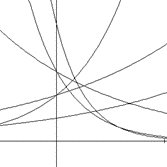
\includegraphics{images/image079.png}

Now we can sketch the derivative. We know a few values for the
derivative function, and on each interval we know the shape we need. We
can use this to create a rough idea of what the graph should look like.

\begin{figure}
\centering
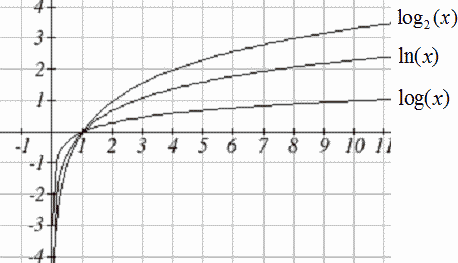
\includegraphics{images/image080.png}
\caption{}
\end{figure}

Smoothing this out gives us a good estimate for the graph of the
derivative.

\begin{figure}
\centering
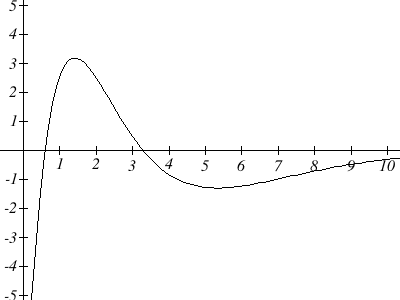
\includegraphics{images/image081.png}
\caption{}
\end{figure}

\begin{longtable}[]{@{}ll@{}}
\toprule
\endhead
\href{section2-7.php}{← Previous Section} & \href{section2-9.php}{Next
Section →}\tabularnewline
\bottomrule
\end{longtable}
